\documentclass{article}

% if you need to pass options to natbib, use, e.g.:
%     \PassOptionsToPackage{numbers, compress}{natbib}
% before loading neurips_2020

% ready for submission
 %\usepackage{neurips_2020}

% to compile a preprint version, e.g., for submission to arXiv, add add the
% [preprint] option:
\usepackage[preprint]{neurips_2020}

% to compile a camera-ready version, add the [final] option, e.g.:
%\usepackage[final]{neurips_2020}https://www.overleaf.com/project/609fb070e16e2310e03cd959

% to avoid loading the natbib package, add option nonatbib:
%\usepackage[nonatbib]{neurips_2020}

\usepackage[utf8]{inputenc} % allow utf-8 input
\usepackage[T1]{fontenc}    % use 8-bit T1 fonts
\usepackage{hyperref}       % hyperlinks
\usepackage{url}            % simple URL typesetting
\usepackage{booktabs}       % professional-quality tables
\usepackage{amsfonts}       % blackboard math symbols
\usepackage{nicefrac}       % compact symbols for 1/2, etc.
\usepackage{microtype}      % microtypography

% Added packages
\usepackage{amsmath,amssymb}

% to insert some figures
\usepackage{graphicx}
\graphicspath{{figs/}}


\title{Policy Optimization with Demonstration}

% The \author macro works with any number of authors. There are two commands
% used to separate the names and addresses of multiple authors: \And and \AND.
%
% Using \And between authors leaves it to LaTeX to determine where to break the
% lines. Using \AND forces a line break at that point. So, if LaTeX puts 3 of 4
% authors names on the first line, and the last on the second line, try using
% \AND instead of \And before the third author name.

\author{%
  Chia-Hung, Liao\\
  Department of Computer Science\\
  National Chiao Tung University\\
  \texttt{aiallen.cs07g@nctu.edu.tw} \\

}

\begin{document}

\maketitle

\section{Introduction}
\label{section:intro}

\begin{itemize}
    \item The main research challenges tackled by the paper: \\
    Exploration still remains a significant challenge to reinforcement learning algorithms, especially the reward signals from the environment are sparse. Learning from demonstrations (LfD) (\cite{hester2018deep,vecerik2017leveraging}) is a common approach for addressing exploration difficulties in sparse reward tasks. However, existing LfD methods is limited by only treating the demonstrations in the same way as self-generated data. Besides, the traditional LfD usually require a large number of high-quality demonstrations which are difficult to collect at scale.
    \item The high-level technical insights into the problem of interest \\
    The intuition of LfD is that the agent could imitate the expert demonstrations when the reward signal sparse in early learning stages instead of random exploration. After acquiring enough assistances, the agent can explore for even better policy on its own. In other words, LfD can be viewed as a dynamic intrinsic reward mechanism. That is, one can introduce demonstrations for reshaping native rewards in RL. Therefore, this research proposes a novel Policy Optimization from Demonstration (POfD) method (\cite{kang2018policy}), which can acquire knowledge from demonstration data to boost exploration, even though the data are scarce and imperfect. 
    \item The main contributions of the paper (compared to the prior works) \\
    1.	The research successfully proves that POfD induces implicit dynamic reward shaping and brings significant benefits for policy improvement.\\
    2.	POfD is generally compatible with most policy gradient algorithms. \\
    3.	It also shows that existing LfD methods \cite{vecerik2017leveraging} can be interpreted as degenerated cases of POfD in terms of how to leverage the demonstration data. 

    \item Your personal perspective on the proposed method \\
    In my opinion, this POfD method looks similar to the inverse reinforcement learning method (IRL) (\cite{fu2017learning}). But the POfD will be better than the typical generative IRL in some sense due to its mechanism. When the environment feedback reward is sparse, we usually let the agent learn from the expert’s demonstration. In addition, we don’t know the reward function for the expert policy. Instead, IRL can adopt generative methods such as generative adversarial networks (GANs) (\cite{goodfellow2014generative}) to learn the reward function for expert policy by using the expert trajectories even though the expert demonstration is few. However, the typical IRL regards expert demonstration as the best policy. When it comes to POfD, it reshapes the reward function during the policy optimization process. Furthermore, POfD does not regard expert demonstration as the best policy. Instead, this new reshaped reward function can guide the agent to imitate expert behavior when the environment reward is sparse, and explore independently when it can get the environment reward value. In this way, the expert demonstration can be more fully utilized, and there is no need to ensure that the expert policy is the optimal one, which is a great improvement compared to the previous methods.
\end{itemize}

\newpage
\section{Problem Formulation}
\label{section:problem}

Please present the formulation in this section. You may want to cover the following aspects:

\begin{itemize}
    \item Your notations (e.g. MDPs, value functions, function approximators,...etc)
    \item The optimization problem of interest
    \item The technical assumptions
\end{itemize}

\subsection{Preliminaries and Notations}

\begin{figure}[htb]
    \center
    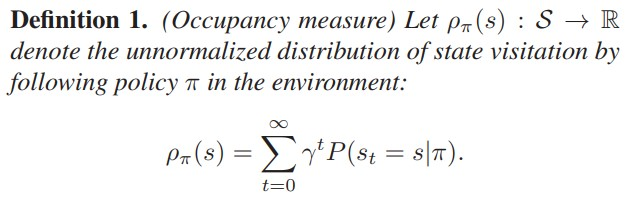
\includegraphics[width=10cm]
    {def1}
    \label{fig: def1}
\end{figure} 

From the Def. 1, for better exploiting demonstrations, this research first converts the expected discounted reward from Eq. (1) to a Eq. (2) defined on occupancy measure (Ho Ermon, 2016). 

\begin{figure}[htb]
    \center
    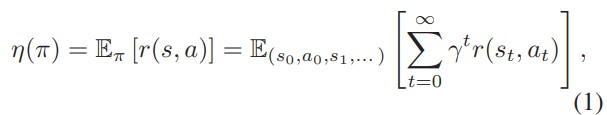
\includegraphics[width=9cm]
    {eq1}
    \label{fig: eq1}
\end{figure} 

\begin{figure}[htb]
    \center
    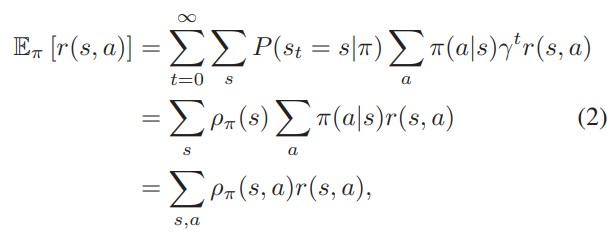
\includegraphics[width=9cm]
    {eq2}
    \label{fig: eq2}
\end{figure} 

In the following lemma (\cite{syed2008game}), the occupancy measure has an important property that it uniquely specifies a policy. 

\begin{figure}[h!]
    \center
    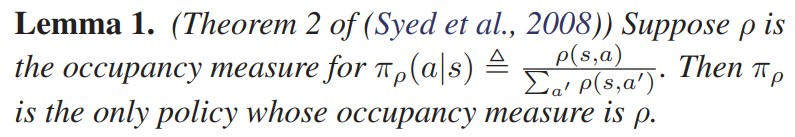
\includegraphics[width=10cm]
    {lemma1}
    \label{fig: lemma1}
\end{figure} 

Besides, in addition to sparse rewards from environments, the agent is also provided with a few demonstrations $D^{E}=\left\{\tau_{1},\tau_{2},...,\tau_{N}\right\}$, where the $i$-th trajectory $\tau_{i}=\left\{(s^{i}_{0},a^{i}_{0}),(s^{i}_{1},a^{i}_{1}),...,(s^{i}_{T},a^{i}_{T}) \right\}$ is generated from executing an unknown expert policy $\pi_{E}$.


\subsection{The optimization problem of interest}

Besides maximizing the expected return $\eta(\pi_{\theta})$ through learning from sparse feedback, this research also encourages the agent to explore by “following” the demonstrations DE. Then an introduce demonstration-guided exploration term $L_{M}(\pi_{\theta},\pi_{E})=D_{JS}(\pi_{\theta},\pi_{E})$ is introduced to the vanilla objective $\eta(\pi_{\theta})$. This gives a new learning objective:

\begin{figure}[h!]
    \center
    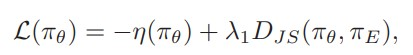
\includegraphics[width=6.5cm]
    {eq3-0}
    \label{fig: eq3-0}
\end{figure} 

Where $\lambda_{1}$ is a trading-off parameter, and $D_{JS}$ is the Jensen-Shannon divergence between current policy $\pi_{theta}$ and the expert one $\pi_{E}$. However, this divergence measure is infeasible since $\pi_{E}$ is unknown. Instead, we redefine the divergence over the occupancy measures $\rho_{\pi}(s,a)$ and $\rho_{\pi_{E}}(s,a)$ by Lemma 1. And finally the proposed demonstration guided learning objective is changed to the Eq. (3)

\begin{figure}[h!]
    \center
    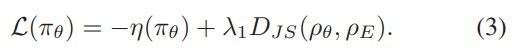
\includegraphics[width=7cm]
    {eq3}
    \label{fig: eq3}
\end{figure} 


\subsection{The technical assumptions}

Although the expert policy may not best one, but its quality is usually better than the agent policy in early training stage. Therefore, this paper presents a reasonable and necessary assumption, and it will be used to prove the benefits of exploration with demonstrations.

\begin{figure}[h!]
    \center
    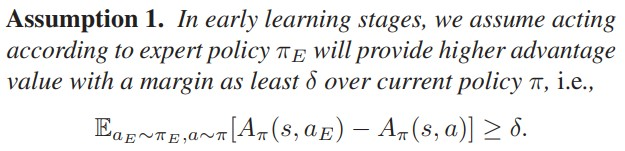
\includegraphics[width=10cm]
    {assump1}
    \label{fig: assump1}
\end{figure} 

And the second assumption is the same when using the form of surrogate objective when proving the TRPO algorithm (\cite{schulman2015trust}).

\begin{figure}[h!]
    \center
    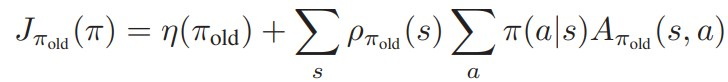
\includegraphics[width=9cm]
    {eq5-1}
    \label{fig: eq5-1}
\end{figure}


The assumption is, the reason why $\rho_{\pi}$ is replaced by $\rho_{\pi_{old}}$ is that the change in state distribution can be ignored due to policy update.

\newpage
\section{Theoretical Analysis}
\label{section:analysis}
Please present the theoretical analysis in this section. Moreover, please formally state the major theoretical results using theorem/proposition/corollary/lemma environments. Also, please clearly highlight your new proofs or extensions (if any).

\subsection{Proof for Benefits of Exploration with Demonstrations}

First, it is quite important to know whether adding the JS-divergence term as learning regularization could improve the agent policy eventually. So, starting from the surrogate function and the learning objective Eq. (3), one can prove the following Theorem:

\begin{figure}[ht]
    \center
    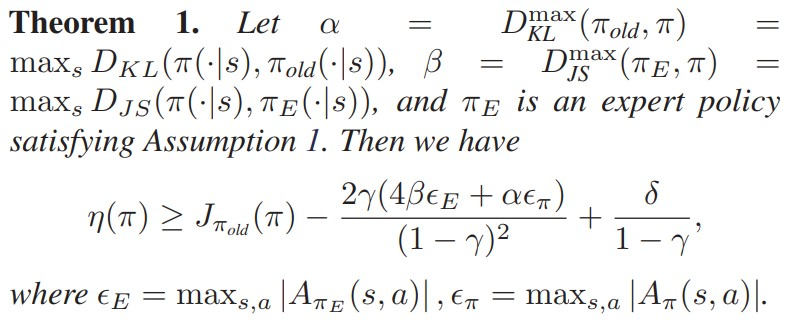
\includegraphics[width=8cm]
    {theorem1}
    \label{fig: theorem1}
\end{figure} 

Since it needs three pages to prove this inequality function of Theorem 1, and it has been provided by the paper’s supplement, so I decide to skip the details in this report. Most importantly, one can use Theorem 1 to further prove the benefits of adding the demonstration guided regularization term. \\
let $M_{i}(\pi)=J_{\pi_{i}}(\pi)-C_{\pi_{E}}D_{JS}^{max}(\pi,\pi_{E})-C_{\pi}D_{KL}^{max}(\pi,\pi_{i})+\hat{\delta}$ \\
where $C_{\pi_{E}}=\frac{8\gamma\epsilon_{E}}{(1-\gamma)^2}$, $C_{\pi}=\frac{2\gamma\epsilon_{\pi}}{(1-\gamma)^2}$, $\hat{\delta}=\frac{\delta}{1-\gamma}$. \\
And substitue the above $M_{i}(\pi)$ into the function of Theorem 1, we can derive:\\ $\eta(\pi_{i+1})\ge M_{i}(\pi_{i+1})$. \\
Then, since the KL divergence between the same policies will be zero, so \\ $\eta(\pi_{i})=M_{i}(\pi_{i})+C_{\pi_{E}}D_{JS}^{max}(\pi_{i},\pi_{E})-\hat{\delta}$. \\
Therefore, from these above two equations, one can derive: \\ $\eta(\pi_{i+1})-\eta(\pi_{i})\ge M_{i}(\pi_{i+1})-M_{i}(\pi_{i})-C_{\pi_{E}}D_{JS}^{max}(\pi_{i},\pi_{E})+\hat{\delta}$ \\
This result recalls the classic monotonic improvement guarantees for the policy gradient algorithm. But POfD brings another two terms $C_{\pi_{E}}D_{JS}^{max}(\pi_{i},\pi_{E})$ and $\hat{\delta}$. This implies when the agent follows the demonstrations, the JS divergence is close to zero, and therefore the advantage  term $\hat{\delta}$ from the reasonable assumption 1 can guarantee the monotonic policy improvement.


\subsection{Main Optimization Objective}

Since the JS divergence is quite hard to optimize, so this paper changes the way to optimize its lower bound which is given as Theorem 2:

\begin{figure}[ht]
    \center
    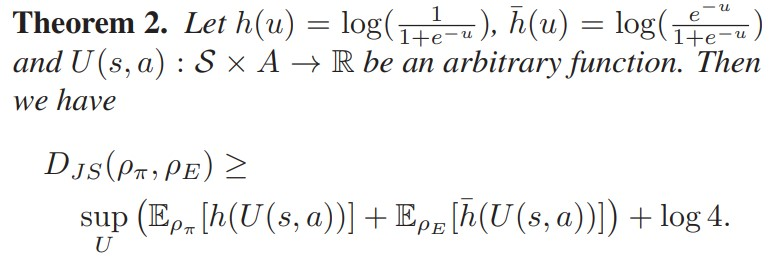
\includegraphics[width=8cm]
    {theorem2}
    \label{fig: theorem2}
\end{figure} 

Also, this theorem has been proved in the supplement provided by the paper author. Therefore, the occupancy measure matching objective can be written as

\begin{figure}[ht]
    \center
    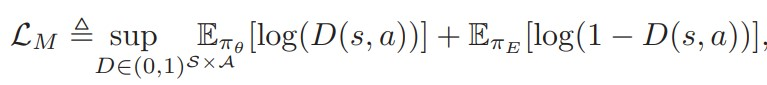
\includegraphics[width=8cm]
    {theorem2-1}
    \label{fig: theorem2-1}
\end{figure} 

That is, the supremum will range over $D(s,a)=\frac{1}{1+e^{-U(s,a)}}$ which is an arbitrary mapping function followed by a sigmoid activation funciton. And this objective can be regarded as the binary classification loss for distinguishing $\pi_{\theta}$ and $\pi_{E}$ w.r.t. state-action pairs sampled from the occupancy measure $\rho_{\theta}$ and $\rho_{E}$.  \\

To avoid the overfitting risks, this paper introduce the causal entropy $-H(\pi_{\theta})$ (\cite{ziebart2010modeling}). And thus the objective becomes the following form:

\begin{figure}[h!]
    \center
    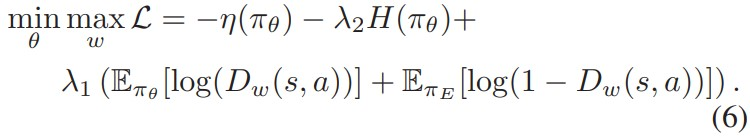
\includegraphics[width=8cm]
    {eq6}
    \label{fig: equation6}
\end{figure} 

It is actually a minimax problem similar to the GANs. In this POfD case, the true distribution is $\rho_{E}$, and the generator is to learn $\rho_{\theta}$. $D$ represents the discriminator parameterized by $w$, and we label the state-action pairs from expert as true ("1") while the policy as false ("0"). 

Moreover, by substituting Eq. (1) and Eq. (2) into Eq. (6), the objective becomes:

\begin{figure}[h!]
    \center
    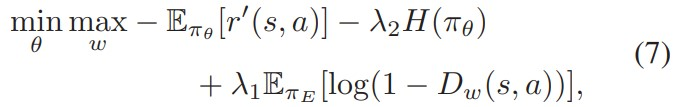
\includegraphics[width=8cm]
    {eq7}
    \label{fig: equation7}
\end{figure}

This function results in a dynamic reward reshaping mechanism. And the reshaped reward function is:   \\
$r^{\prime}(s,a)=r(s,a)-\lambda_{1}log(D_{w}(s,a))$ \\

It can augment the environment reward with aid of demonstrations. In other words, when the environment feedback is sparse, this reshaped reward can force the policy to generate similar trajectory as $\pi_{E}$. So, such way can make the agent to explore the environment more efficiently.

\subsection{POfD Algorithm}

The Eq. (7) can be optimized by alternately updating the parameters $w$ and $\theta$ of the discriminator and the agent policy, respectively. The overall optimization details are summarized in Alg. 1.
\begin{figure}[h!]
    \center
    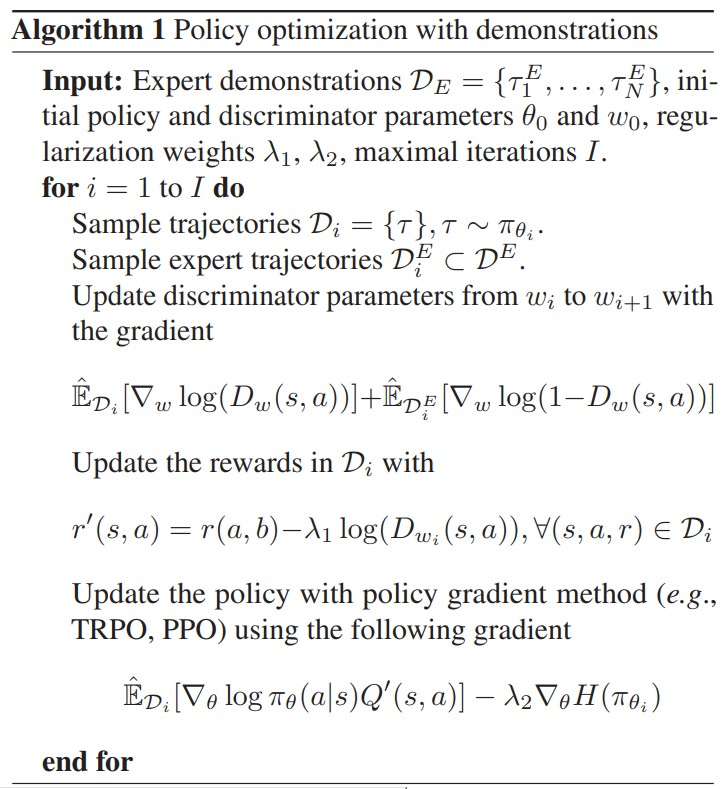
\includegraphics[width=7.5cm]
    {algorithm}
    \label{fig: algorithm}
\end{figure} 

Note that the reshaped policy gradient is given by:
\begin{figure}[h!]
    \center
    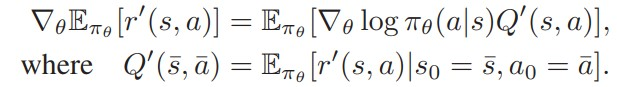
\includegraphics[width=8cm]
    {reshapeR}
    \label{fig: reshapeR}
\end{figure} 

And the gradient of causal entropy is:
\begin{figure}[h!]
    \center
    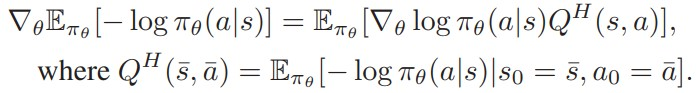
\includegraphics[width=8cm]
    {causalH}
    \label{fig: causalH}
\end{figure} 







\section{Conclusion}
\label{section:conclusion}
Please provide succinct concluding remarks for your report. You may discuss the following aspects:
\begin{itemize}
    \item The potential future research directions 
    \item Any technical limitations 
    \item Any latest results on the problem of interest 

Observing the new reward function $r^{\prime}(s,a)$  in Eq. (7), we can find that if the environment feedback rewards are very sparse, then the agent behaves like an expert, which can guide the agent to learn from the expert; but when the environment itself has rewards, it is directly Relying on these environment rewards itself for learning, not relying on expert demonstrations. Therefore, it realizes learning experts first and then self-learning. \\
However, the optimization problem of POfD begins with the demonstration guided regularization term which is a typical JS-divergence, and then is deduced into the form similar to GANs. As I know, the GAN method with the original JS-divergence-based objective is usually hard to be optimized and converge. So this POfD may have similar technical limitations like the early type of GAN, maybe it can refer to the subsequent developments of GAN to find a more useful technique to further finetune its current optimization method and get even better performance.

    
    
\end{itemize}





{
\small
\bibliographystyle{apalike}
\bibliography{reference}
}



\end{document}
